% !TeX program = xelatex
% 课堂展示用汇报稿，内容参考 docs/总体报告/[SE]4_总体报告v1.0.pdf
\documentclass[UTF8,aspectratio=169]{ctexbeamer}

\usepackage{zju}
\usepackage{amsmath}
\usepackage{booktabs}
\usepackage{graphicx}
\usepackage{hyperref}
\usepackage{xcolor}
\usepackage{tikz}

\graphicspath{
    {./}
    {../figure/}
    {../../总体设计报告/figures/exported/}
    {../../总体设计报告/figures/ui/}
    {../../测试文档/screenshots/}
    {../../设计模式报告/figures/exported/}
}

\beamertemplateballitem
\setbeamertemplate{navigation symbols}{}
\setbeamerfont{frametitle}{size=\large,series=\bfseries}
\setbeamerfont{itemize/enumerate body}{size=\small}
\setbeamerfont{itemize/enumerate subbody}{size=\footnotesize}
\setbeamerfont{block body}{size=\small}
\setbeamerfont{caption}{size=\scriptsize}

\definecolor{ZJUBlue}{RGB}{0,63,136}
\definecolor{GoodGreen}{RGB}{28,135,92}
\definecolor{WarmOrange}{RGB}{218,129,38}

\title[总体报告展示]{校园学术活动智能推荐平台}
\subtitle{总体报告课堂展示}
\author[SE 第4组]{黄晗 \quad 宫上珺 \quad 孟祥烨 \\ 李妍雅 \quad 庞星磊 \quad 朱致远}
\institute[浙江大学]{}
\date[2026-06]{2026 年 6 月}

\newcommand{\keyword}[1]{\textcolor{ZJUBlue}{\textbf{#1}}}
\newcommand{\good}[1]{\textcolor{GoodGreen}{\textbf{#1}}}

\begin{document}

\begin{frame}
    \titlepage
\end{frame}

\section{项目定位}

\begin{frame}{项目定位：从“发现活动”到“安排日程”的完整流程}
    \begin{columns}[T,onlytextwidth]
        \begin{column}{0.48\textwidth}
            \begin{block}{问题背景}
                \begin{itemize}
                    \item 校园学术活动发布渠道分散，学生需要反复浏览不同通知入口。
                    \item 活动字段格式不统一，检索、筛选和判断价值的成本较高。
                    \item 活动是否与课程或已有安排冲突，通常需要手工对照课表。
                    \item 活动数据需要兼顾爬虫采集、人工维护和后续质量管理。
                \end{itemize}
            \end{block}
        \end{column}
        \begin{column}{0.48\textwidth}
            \begin{block}{系统目标}
                \begin{itemize}
                    \item 建设统一的活动信息入口，支持活动聚合、搜索和详情查看。
                    \item 基于兴趣标签、热度、时间和冲突信息提供可解释推荐。
                    \item 导入课程表，加入活动日程前自动检测时间冲突。
                    \item 为管理员提供活动维护、OCR 辅助录入和爬虫记录管理能力。
                \end{itemize}
            \end{block}
        \end{column}
    \end{columns}
\end{frame}

\begin{frame}{总体流程图：用户流程、数据管道与存储机制}
    \centering
    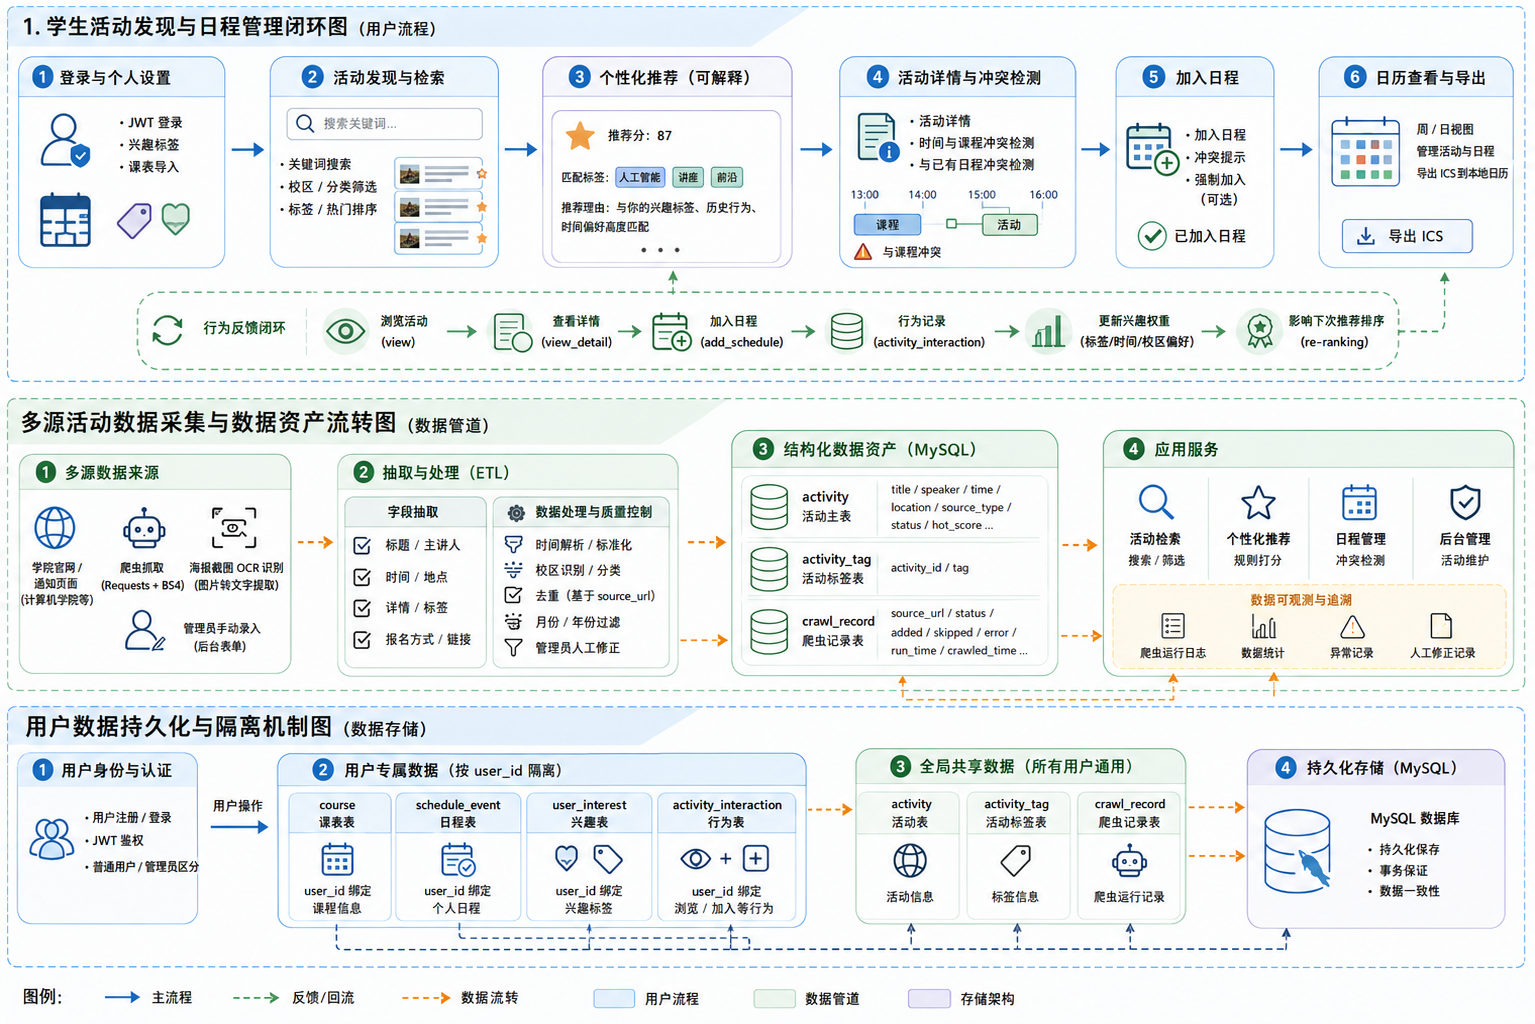
\includegraphics[width=1.06\linewidth,height=0.84\textheight,keepaspectratio]{总图.png}
\end{frame}

\begin{frame}{功能实现}
    \small
    \begin{tabular}{p{0.18\linewidth}p{0.56\linewidth}p{0.16\linewidth}}
        \toprule
        \textbf{模块} & \textbf{主要能力} & \textbf{状态} \\
        \midrule
        数据采集与处理 & 手动录入、爬虫抓取、OCR 辅助识别、清洗去重、结构化入库 & \good{已完成} \\
        推荐与检索 & 关键词搜索、分类/校区/标签筛选、热门排序、规则推荐与推荐理由 & \good{已完成} \\
        日程协同 & 课程导入、课程展开、活动加入日程、冲突检测、自定义日程、ICS 导出 & \good{已完成} \\
        后台管理 & 管理员登录、活动新增/编辑/下架、统计查看、爬虫记录查询 & \good{已完成} \\
        学术沉淀 & 个人中心、兴趣标签展示、活动行为记录、学术轨迹基础数据 & \good{基础可用} \\
        \bottomrule
    \end{tabular}

    \vspace{0.8em}
    \begin{block}{主流程}
        学生端：登录或匿名浏览活动 $\rightarrow$ 查看推荐/列表 $\rightarrow$ 进入详情 $\rightarrow$ 检测冲突 $\rightarrow$ 加入日程 $\rightarrow$ 日历查看与 ICS 导出。
    \end{block}
\end{frame}

\section{总体设计}

\begin{frame}{技术框架}
    \centering
    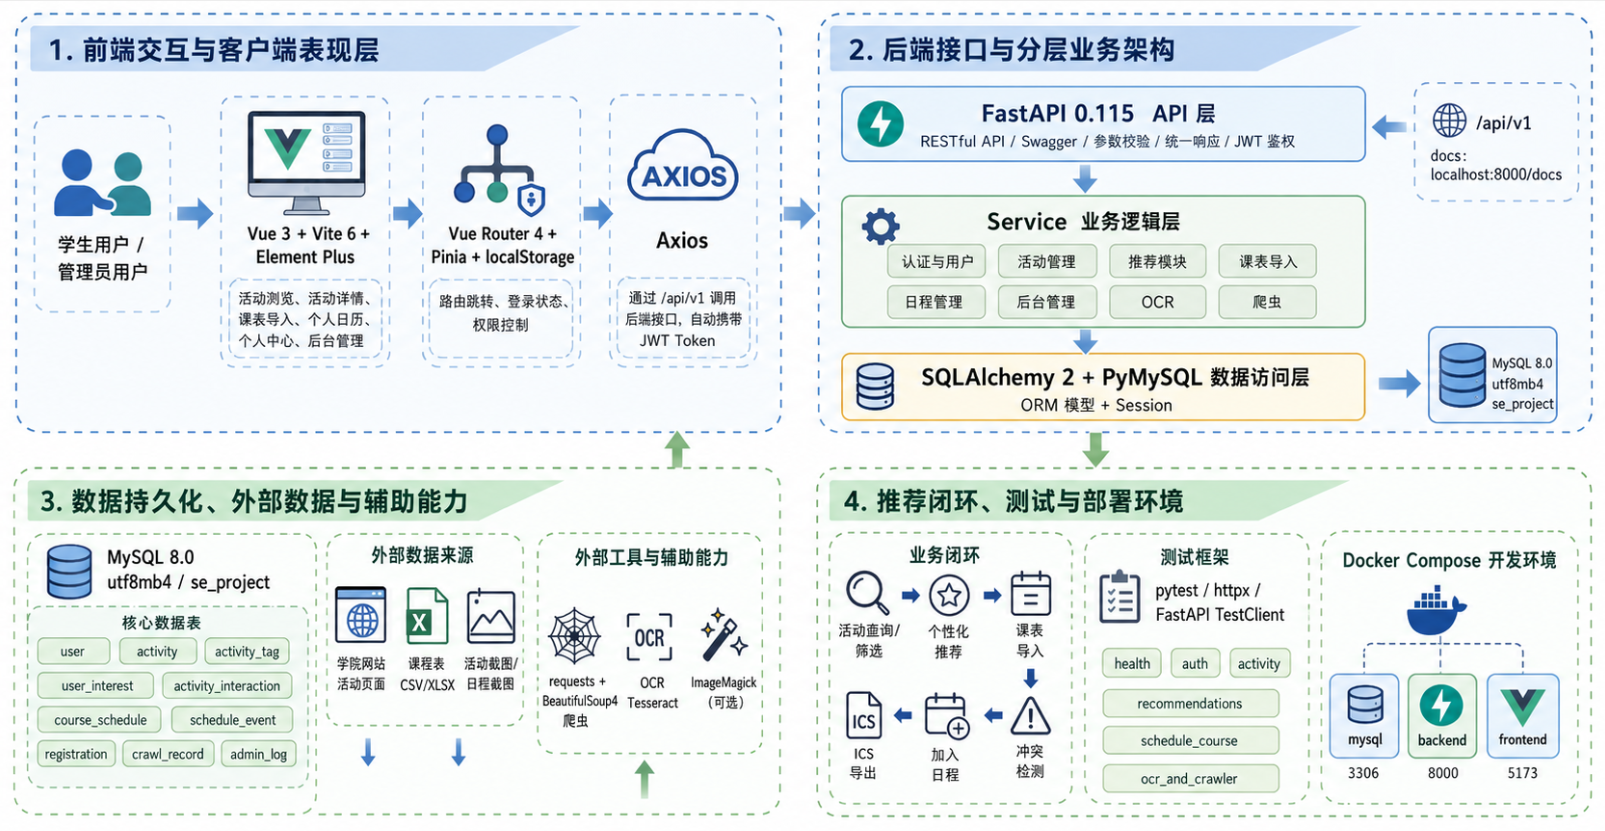
\includegraphics[width=1.04\linewidth,height=0.82\textheight,keepaspectratio]{技术框架.png}
\end{frame}

\section{测试与总结}

\begin{frame}{测试结果：核心功能通过自动化与页面验证}
    \begin{columns}[T,onlytextwidth]
        \begin{column}{0.36\textwidth}
            \begin{itemize}
                \item 覆盖登录注册、活动浏览、推荐、课程导入、日程与后台管理等模块。
                \item 接口统一返回 \texttt{\{code, message, data\}}，便于前端处理和自动化断言。
                \item 关键页面保留截图，支撑课堂验收展示。
            \end{itemize}
        \end{column}
        \begin{column}{0.60\textwidth}
            \scriptsize
            \renewcommand{\arraystretch}{1.08}
            \begin{tabular}{p{0.22\linewidth}p{0.48\linewidth}p{0.16\linewidth}}
                \toprule
                \textbf{模块} & \textbf{验证内容} & \textbf{结论} \\
                \midrule
                登录与权限 & 登录、注册、当前用户、后台权限 & \good{通过} \\
                活动浏览 & 列表分页、详情、搜索筛选、交互记录 & \good{通过} \\
                个性化推荐 & 通用推荐、登录推荐、后台预览 & \good{通过} \\
                课程导入 & 新增课程、CSV/XLSX 导入、删除 & \good{通过} \\
                日程与冲突 & 日程查询、冲突检测、强制加入、ICS 导出 & \good{通过} \\
                后台管理 & 新增、编辑、下架活动、统计查看 & \good{通过} \\
                OCR 与爬虫 & OCR 预览、异常输入、抓取记录查询 & \good{通过} \\
                \bottomrule
            \end{tabular}
            \vspace{0.25em}
            \begin{block}{测试结论}
                \scriptsize
                结项版本已覆盖从活动发现、推荐、课程导入、冲突检测到后台维护的主流程，测试结果与页面截图共同证明核心流程可运行。
            \end{block}
        \end{column}
    \end{columns}
\end{frame}

\begin{frame}{总结与展望}
    \begin{columns}[T,onlytextwidth]
        \begin{column}{0.48\textwidth}
            \begin{block}{项目成果}
                \begin{itemize}
                    \item 建立统一活动数据模型和接口规范。
                    \item 完成可解释推荐、搜索筛选、课程导入、冲突检测和 ICS 导出。
                    \item 建立管理员后台，支持活动维护、OCR 辅助录入和爬虫记录查看。
                    \item 形成需求、总体设计、设计模式和测试等配套文档。
                \end{itemize}
            \end{block}
        \end{column}
        \begin{column}{0.48\textwidth}
            \begin{block}{后续优化}
                \begin{itemize}
                    \item 引入更细粒度用户画像和点击反馈，优化推荐权重。
                    \item 扩展更多学院活动来源，完善爬虫失败重试和字段质量检查。
                    \item 增强日历体验，支持通勤时间提醒和更灵活的 ICS 同步。
                    \item 补充端到端测试、兼容性测试和部署安全加固。
                \end{itemize}
            \end{block}
        \end{column}
    \end{columns}
\end{frame}

\end{document}
